\documentclass{article}
\usepackage{graphicx}
\usepackage[utf8]{inputenc}
\usepackage{polski}
\usepackage[backend=biber]{biblatex}
\usepackage{indentfirst}
\usepackage{hyperref}
\usepackage{graphicx}
\usepackage{mathrsfs}
\usepackage{amssymb}
\usepackage{amsmath}

\addbibresource{bib_cite.bib}

\begin{document}

\title{Regresja zmian cen akcji}
\author{Karol Oleszek}

\maketitle
\newpage
\tableofcontents

\newpage
\section{Wstęp}
Przewidywanie zmian cen akcji oraz innych instrumentów finansowych znajduje się w centrum zainteresowania inwestorów. Zmiany cen są podstawowym zjawiskiem powodującym bogacenie się lub ubożenie inwestora indywidualnego bądź instytucjonalnego, dlatego też próby zrozumienia i opisania reguł rządzących tym zjawiskiem są kluczowe dla podejmowania skutecznych decyzji o alokacji kapitału.

Teoria rynków kapitałowych proponuje wiele różnych wyjaśnień zmienności cen: hipoteza rynku efektywnego (\textcite{Bachelier1900}) zakłada, że ceny rynkowe akcji w danej chwili odzwierciedlają wszystkie dostępne informacje o spółce; autorzy i zwolennicy hipotezy krótkoterminową zmienność cen opisują jako losowy ruch wokół efektywnej wartości. Hipoteza rynku efektywnego znalazła wielu zwolenników, którzy poddawali w wątpliwość samą zasadność przewidywania cen (\textcite{Cowles1932}), jak również zainspirowała powstanie indeksowych funduszy inwestycyjnych.

Hipoteza rynku efektywngeo spotkała się z szeroką krytyką ze strony ekonomistów i inwestorów giełdowych, którzy wskazywali na kontrprzykłady obalającę hipotezę. Współcześnie właściwie wszystkie duże organizacje finansowe używają różnego rodzaju systematycznych narzędzi do analizy i prognozy zmian cen na rynkach kapitałowych (\textcite{GCM2013}). Duże oraz wciąż rosnące znaczenie ma też algorytmiczny handel (\textcite{Capgemini2012}).

Do złożonego problemu jakim jest symulacja i prognostyka zachowania rynków kapitałowych stosuje się bardzo szeroki wachlarz metod statystycznych, algorytmicznych i ekonometrycznych. Duże zastosowanie mają metody uczenia maszynowego (\textcite{ShenJiangZhang2012}), w tym głebokie sieci neuronowe o niekonwencjonalnych architekturach. Ponadto do prognostyki coraz częściej używa się analizy języka naturalnego (\textcite{WangHoLin2018}).

Poniższa praca zawiera przekrojową regresję zmian cen akcji na rynku amerykańskim w 2019 z wykorzystaniem standardowych narzędzi ekonometrycznych. Zbiór danych służący do konstrukcji modelu zawiera dane z roku 2018, dotyczące sytuacji finansowych, kapitałowych i operacyjnych spółek, zawarte w formie wskaźników i pozycji ze sprawozdań finansowych.

\newpage
\section{Cel projektu}

\subsection{Model wyboru akcji do celów inwestycyjnych}
Celem projektu jest wyznaczenie bazowego poziomu efektywności wyboru spółek, których akcje w nadchodzącym roku zyskają na wartości. Za wybór odpowiadał będzie model, który powstanie przy użyciu metody najmniejszych kwadratów i który będzie mógł służyć jako punkt odniesienia do badania efektywności innych metod predykcji.

Efektywność prognostyczna modelu zostanie zbadana przy użyciu \textit{średniego absolutnego błędu prognozy ex post}, danego wzorem:

\[ MAE = \frac{1}{s} \sum_{t=1}^{s} | y_t - y_t^P | \],

Gdzie:

~$s$ - ilość obserwacji w testowym zbiorze danych

~$y_t$ - prawdziwa wartość zmiennej objaśnianej

~$y_t^P$ - prognozowana wartość zmiennej objaśnianej

\medskip

\subsection{Zbadanie zależności pomiędzy zmianą cen, a informacjami finansowymi}
Ponadto model posłuży do oceny wpływu informacji finansowych zawartych w publicznie dostepnych źródłach na przyszłą wartość spółek giełdowych. Ocena ta może być użyteczna przy podejmowaniu decyzji o tym, jakie dane zbierać na temat spółek w celu skutecznego przewidywania ich przyszłej wyceny.

Miarą tej oceny będzie współczynnik determinacji ~$R^2$, dany wzorem:

\[ R^2 = \frac{\sum_{t=1}^{n}(y_t^P-\overline{y})^2}{\sum_{t=1}^{n}(y_t-\overline{y})^2} \],

Gdzie:

~$n$ - ilość obserwacji w uczącym zbiorze danych

~$y_t$ - prawdziwa wartość zmiennej objaśnianej

~$y_t^P$ - prognozowana wartość zmiennej objaśnianej

~$\overline{y}$ - średnia arytmetyczna zmiennej objaśnianej

\newpage
\section{Opis danych}

\subsection{Zbiór danych}
Zbiór danych użyty w projekcie pochodzi z internetowej platformy \href{https://www.kaggle.com/cnic92/200-financial-indicators-of-us-stocks-20142018}{Kaggle} (\textcite{Carbone2019}). Zawiera on zmienną objaśnianą ~$Y$ - procentową zmianę ceny akcji danej spółki w 2019 roku, oraz zmienne objaśniające ~$X_i,  i=1\dots k$ - k-1 wskaźników finansowych i pozycji z formularza \textit{10-K}\footnote{\textit{Form 10-K} jest to coroczne podsumowanie finansowe składane przez amerykańskie spółki giełdowe do \textit{U.S. Securities and Exchange Commission}, federalnej agencji nadzoru finansowego.}, a także zmiennej kategorycznej oznaczającej sektor gospodarki rozważanej spółki.

\subsection{Usuwanie braków danych}
Dane zostały zebrane przy użyciu interfejsu programistycznego \textit{Financial Modeling Prep API} i zawierały pewne braki wynikające z różnic w dokumentach źródłowych. Dla celów analizy usunięte zostały wszystkie obserwacje, w których brakowało więcej niż 50 wartości oraz wszystkie zmienne, w których co najmniej 10\% obserwacji nie miało przypisanej wartości. Po tej transformacji, w zbiorze danych pozostało 4122 obserwacji oraz 179 zmiennych (4392 x 222, 9,98\% braków przed transformacją). Wciąż brakujące 0,82\% wartości zostało zastąpionych średnimi arytmetycznymi odpowiednich zmiennych.

\subsection{Transformacja zmiennej kategorycznej}
Kategoryczna zmienna objaśniająca \textit{Sector}, która przyjmowałą 11 różnych wartości (Consumer Cyclical, Energy, Technology, Industrials, Financial Services, Basic Materials, Communication Services, Consumer Defensive, Healthcare, Real Estate, Utilities) została przekształcona na 10 zmiennych zero-jedynkowych. Po tej operacji zbiór danych składał się ze 188 zmiennych.

\subsection{Zmienne objaśniające}
Zbiór danych składa się z grupy zmiennych opisujących realne wielkości ze sprawozdań finansowych wyrażone w dolarach amerykańskich np. zysk brutto, wydatki na badania i rozwój. Na drugą grupę zmiennych składają się wskażniki finansowe, będące często przekształconymi zmiennymi z pierwszej grupy, wyrażone jako stosunek różnych wielkości np. zysk na akcję, wzrost zysku w ciągu roku. Trzecia grupa zmiennych to przekształcona zmienna \textit{Sector}. Ze względu na liczbę zmiennych pełna lista zmiennych wraz ze statystykami znajduje się w załączniku do pracy.

\newpage
\subsection{Rozkład zmiennej objaśnianej}
Zmienna objaśniana ~$Y$ to wyrażona w procentach zmiana ceny akcji spółki w roku 2019. Przyjmuje ona wartości -99,86\% do +3756,72\%. Większa część wartości jest większa od zera co wskazuje na pozytywną bazową efektywność tzw. strategii \textit{buy and hold}, która polega na zakupie akcji, a następnie oczekiwaniu na wzrost jej wartości.

\begin{table}[h!]
    \begin{center}
    \begin{tabular}{|c | c|} 
    \hline
    Statystyka & Wartość \\
    \hline\hline
    Średnia arytmetyczna & 21,15 \\ 
    \hline
    Odchylenie standardowe & 84,93 \\
    \hline
    Kwartyl dolny & -9,30 \\
    \hline
    Mediana & 17,83 \\
    \hline
    Kwartyl górny & 40,92 \\
    \hline
    Wartość najmniejsza & -99,86 \\
    \hline
    Wartość największa & 3756,71 \\
    \hline
   \end{tabular}
    \end{center}
   \caption{Statystyki - zmienna objaśniana}
\end{table}

\begin{figure}[h!]
    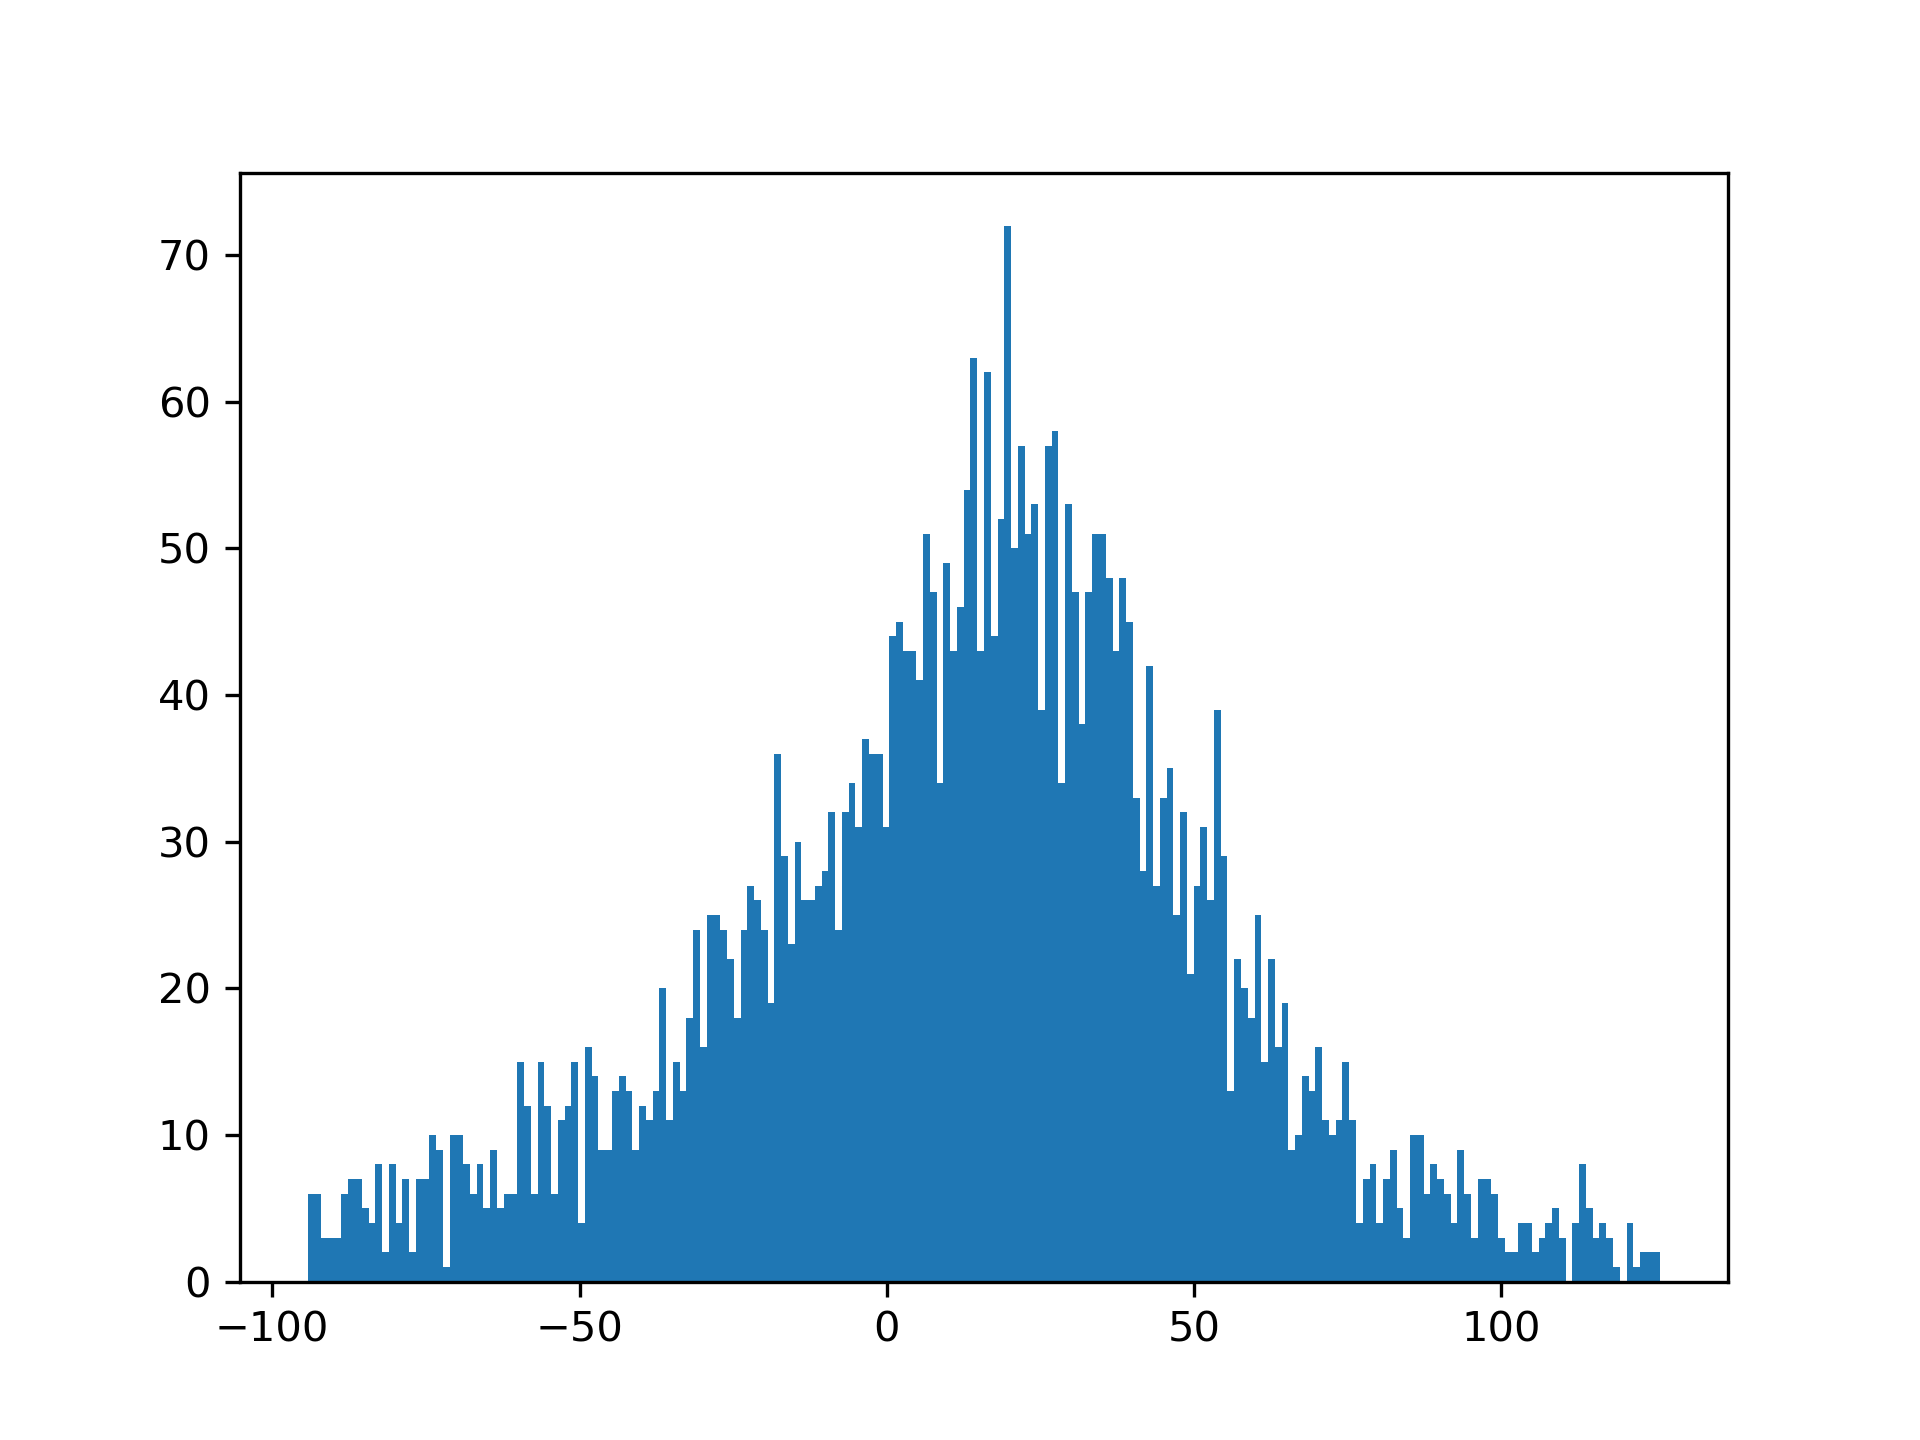
\includegraphics[width=\linewidth]{source/YHistogram.png}
    \caption{Histogram zmiennej objaśnianej}
\end{figure}

\newpage
\subsection{Korelacja}
Korelacja zmiennej objaśnianej ze zmiennymi objaśnianymi jest bardzo słaba, co wskazuje na potencjalnie silnie nieliniowy charakter zachodzących zależności.
\begin{table}[h!]
    \begin{center}
    \begin{tabular}{|c | c|} 
    \hline
    Statystyka & Wartość \\
    \hline\hline
    Średnia arytmetyczna & 0.0006535276131026212 \\ 
    \hline
    Odchylenie standardowe & 0.01430737685985159 \\
    \hline
    Kwartyl dolny & -0.006560508005214499 \\
    \hline
    Mediana & 0.0009029552423272379 \\
    \hline
    Kwartyl górny & 0.008516164727314403 \\
    \hline
    Wartość najmniejsza & -0.07707504123521973 \\
    \hline
    Wartość największa & 0.04058496958769639 \\
    \hline
    \end{tabular}
    \end{center}
   \caption{Korelacja zmiennej objaśnianej ze zmiennymi objaśnianymi}
\end{table}

\begin{figure}[h!]
    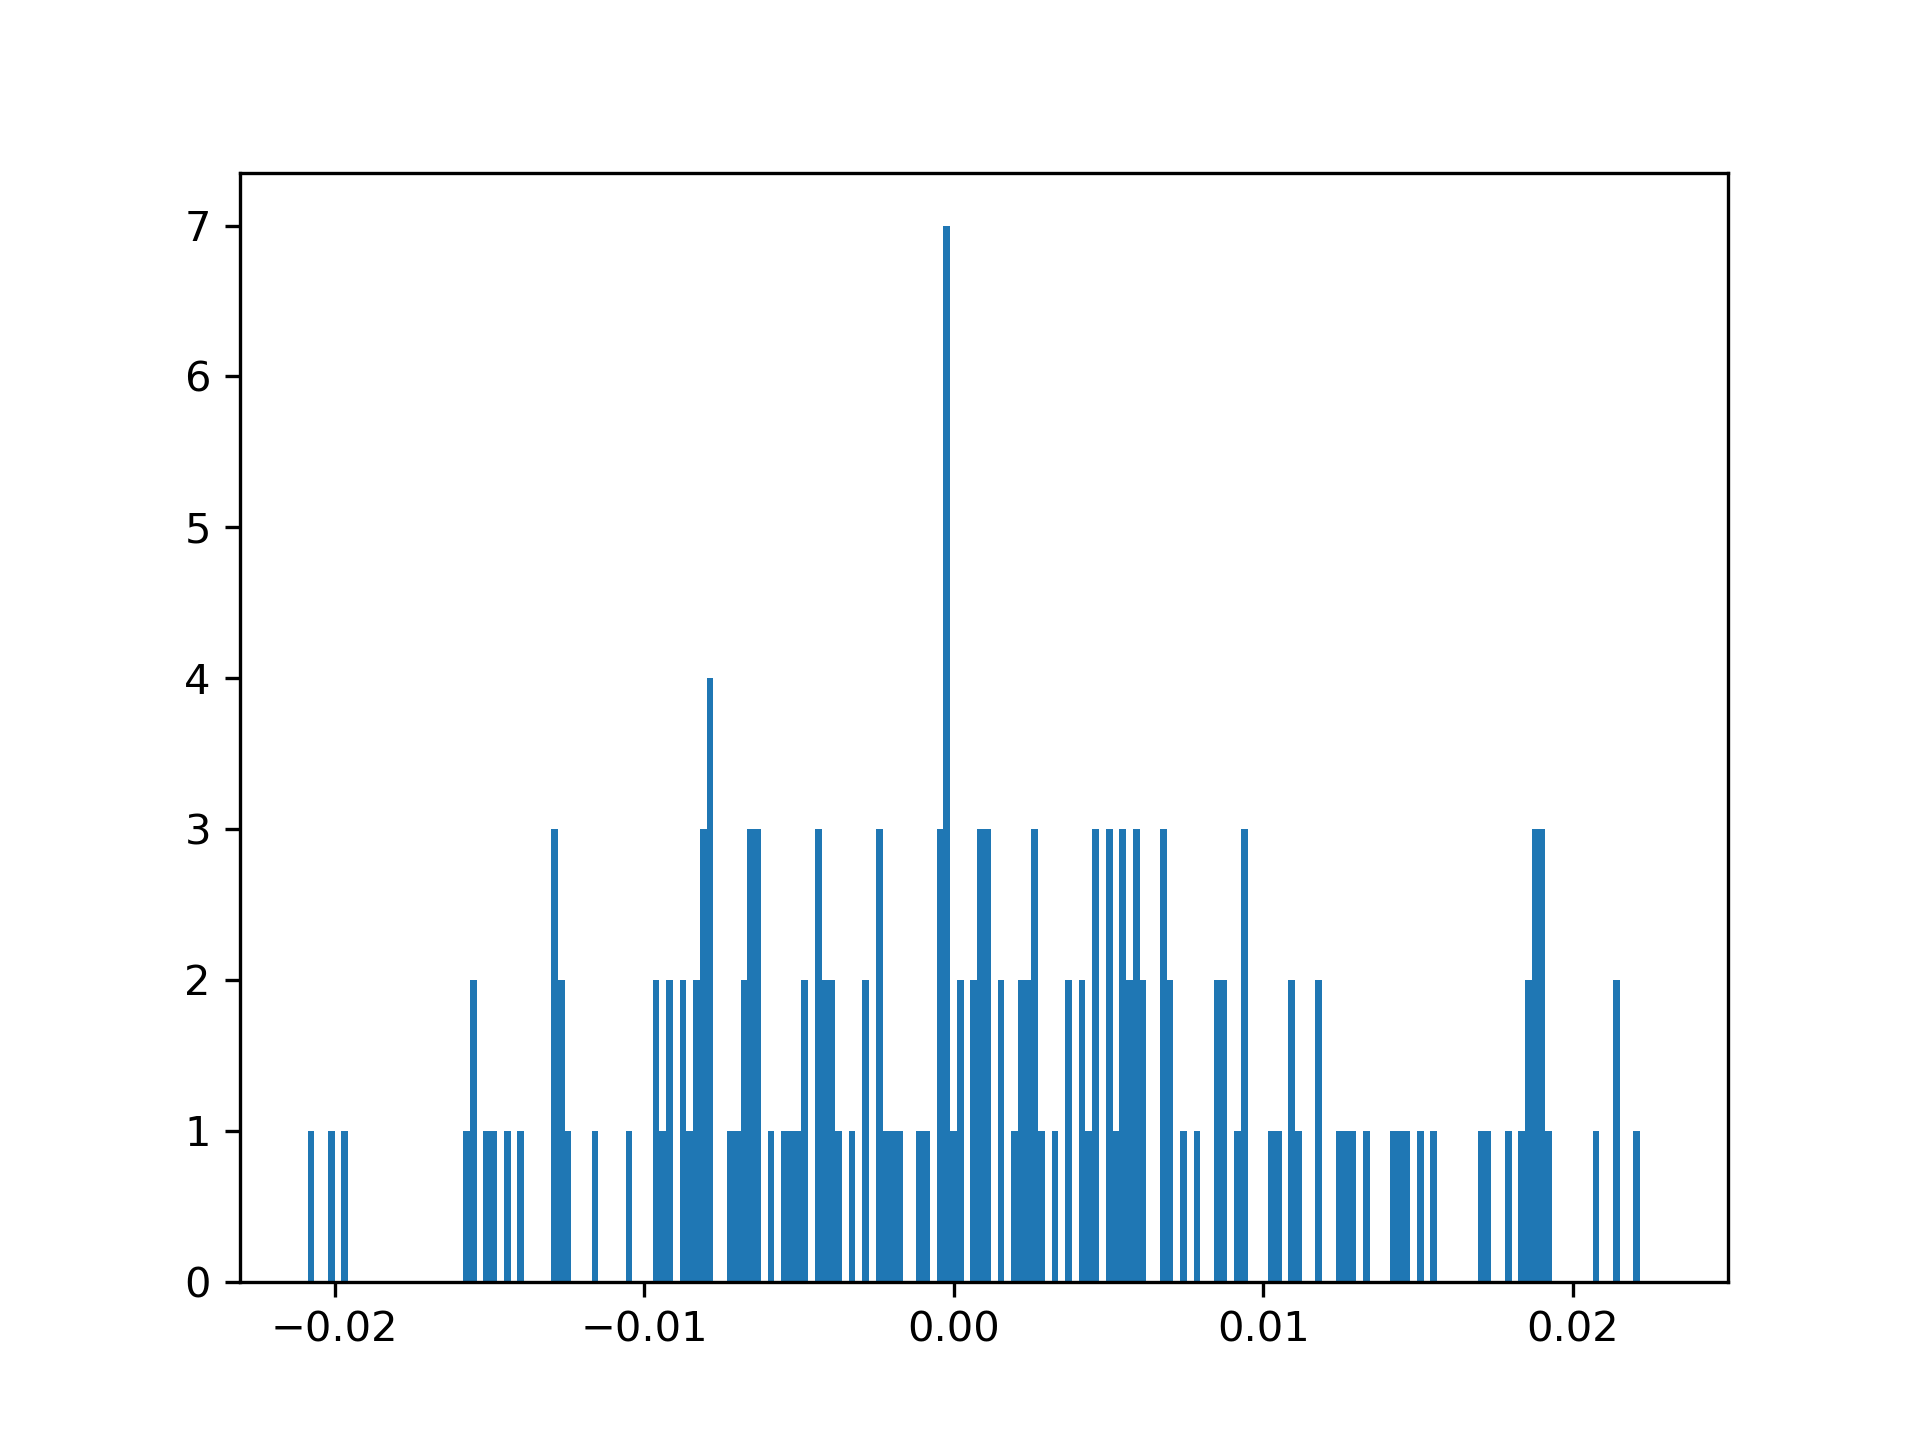
\includegraphics[width=\linewidth]{source/CorrHist.png}
    \caption{Histogram korelacji zmiennej objaśnianej ze zmiennymi objaśnianymi}
\end{figure}

\newpage
Korelacja pomiędzy niektórymi zmiennymi objaśniającymi jest silna, co można wyjaśnić zależnościami pomiędzy rozmiarem spółki, a wielkościami w \textit{10-K Form}. Nie wszystkie bazowe zmienne objaśniające mogą znaleźć się w modelu, ponieważ spowodowałoby to wystąpienie zjawiska współliniowości.
\begin{figure}[h!]
    \includegraphics[width=\linewidth]{source/CorrelationMatrix.png}
    \caption{Macierz korelacji}
\end{figure}

\subsection{Podział zbioru danych}
Zbiór danych podzielony jest na dane treningowe(90\%) użyte do estymacji parametrów modelów oraz dane testowe(10\%) służące do oceny prognozy \textit{ex post}.

\newpage
\section{Wybór postaci modelu oraz dobór zmiennych do modelu}
\subsection{Specyfikacja kryteriów}
Praca odpowiada na dwa pytania:
\begin{enumerate}
    \item Jaka jest bazowa efektywność predykcji?
    \item Jaki jest wpływ informacji zawartych w rozważanych danych na zmiany cen akcji?
\end{enumerate}

Odpowiedzią na pierwsze pytanie jest efektywność modelu o najlepszych właściwościach prognostycznych.

Odpowiedzią na drugie pytanie jest ocena współczynnika determinacji poprawnie zweryfikowanego modelu ekonometrycznego.

\subsection{Rozważana klasa funkcji}
Modele wybrane są z klasy funkcji dopuszczalnych ~$\mathscr{F}: \mathbb{R^K\to R}$,
gdzie K: liczba zmiennych w zbiorze danych.

Funkcje przyjmują analityczną postać:

~$\hat{Y}=a_0+a_1*X_1+...+a_k*X_k$;

parametry szacowane są przy użyciu metody najmniejszych kwadratów.

Ze względu na potencjalnie nielinowy charakter zależności rozważony został zbiór danych rozszerzony o przetransformowane zmienne: ~$e^{\frac{X_i-\overline{X_i}}{\sigma_{X_i}}}, X_i^2, X_i^3$ o łącznym rozmiarze 4392 x 748. Dalsze rozszerzanie zbioru danych osłabiło by stabilność numeryczną modeli i nadmiernie zwiększyło by wymiar Wapnika-Czerwonienkisa, co osłabiło by możliwości generalizacji przez modele (\textcite{Kaminski2017}).

\newpage
\subsection{Rozważany podzbiór funkcji}
Ze względu na ilość zmiennych, użycie metody o wykładniczej złożoności obliczeniowej, np. metody Hellwiga, byłoby nieefektywne. W związku z tym rozważany jest K-elementowy zbiór funkcji wyłoniony przy użyciu uproszczonej \textit{metody krokowej wstecz}. Rozważany jest model ze wszystkimi zmiennymi, a następnie z modelu usuwana jest najmniej istotna statystycznie zmienna. Procedura jest powtarzana dopóki w modelu jest więcej niż jedna zmienna. Dla celów stworzenia podzbioru funkcji nie jest sprawdzana normalność rozkładu resztowego.

\subsection{Kryterium wyboru modelu prognostycznego}
Spośród rozważanego podzbioru funkcji wybrana jest funkcja z najmniejszym \textit{absolutnym błędem prognozy ex post} oszacowanym przy użyciu sprawdzianu krzyżowego na danych treningowych.

Sprawdzian krzyżowy polega na podziale zboriu danych na J podzbiorów, a następnie wykonaniu J ocen błędu prognozy(za każdym razem inny podzbiór jest uznawany za testowy, J-1 podzbiorów treningowych) i obliczeniu ich średniej.

\[\hat{MAE}= \frac{1}{J} \sum_{t=1}^{J} ( MAE_i ) \]

\subsection{Kryterium wyboru modelu analitycznego}
Spośród rozważanego podzbioru funkcji wybrana jest funkcja z najwyższym skorygowanym współczynnikiem determinacji ~$R^2$, która została poprawnie zweryfikowana. W przypadku wystąpienia niepożadanych zjawisk w modelu, rozważany podzbiór funkcji powiększony zostaje o model z zastosowanymi stosownymi korektami.


\newpage
\section{Weryfikacja poprawności modelu}
Poniżej opisane są procedury weryfikacji poprawności modelu oszacowanego metodą najmniejszych kwadratów. Przyjęty poziom istotności ~$\alpha=0,05$.

\subsection{Współliniowość}
Wyznaczamy k modeli MNK, gdzie zmienną objaśnianą jest jedna ze zmiennych objaśniających, a zmiennymi objaśniającymi pozostałe zmienne. Wyznaczamy k współczynników determinacji; jeżeli którykolwiek z nich większy jest niż 0,9 , to w modelu występuje niepożądane zjawisko współiniowości zmiennych.

\subsection{Koincydencja}
Jeżeli dla każdego i=1..k:
\[sgn(r_i) = sgn(a_i)\],

gdzie:

~$r_i$: korelacja pomiędzy zmienną objaśnianą, a i-tą zmienną objaśniającą.

~$a_I$: oszacowany i-ty parametr modelu.

to model jest koincydentny. Koincydencja modelu jest pożądaną cechą.

\subsection{Efekt katalizy}
Niech ~$(X_i, X_j)$ będzie regularną parą korelacyjną. Wówczas jeżeli ~$r_{ij} < 0$ lub ~$r_{ij} > \frac{r_i}{r_j}$, gdzie:

~$r_{ij}$: korelacja między i-tą, a j-tą zmienną objaśniającą.

to zmienna ~$X_i$ jest katalizatorem. Poprawny model nie zawiera katalizatorów.

\newpage
\subsection{Normalność rozkładu reszt}
Normalność rozkładu składnika resztowego modelu jest cechą niezbędną do poprawnej interpretacji m.in. testów istotności parametrów modelu. Normalność rozkładu można zbadać przy użyciu testu Jarque-Bera.

~$H_0$: składnik losowy modelu ma rozkład normalny.

~$H_1$: składnik losowy modelu nie ma rozkładu normalnego.

Statystyka testowa ~$JB$ ma rozkład ~$\chi^2$ o dwóch stopniach swobody.

\[JB=\frac{n-k}{6}(A^2+\frac{1}{4}(K-3)^2)\],

gdzie:

Współczynnik skośności:
\[A = \frac{\hat{\mu}_3}{\hat{\sigma}^3} = 
\frac{\frac{1}{n} \sum_{t=1}^{n} ( x_t - \overline{x} )^3}
{(\frac{1}{n} \sum_{t=1}^{n} ( x_t - \overline{x} )^2)^{\frac{3}{2}}}
\]

Kurtoza:
\[K = \frac{\hat{\mu}_4}{\hat{\sigma}^4} = 
\frac{\frac{1}{n} \sum_{t=1}^{n} ( x_t - \overline{x} )^4}
{(\frac{1}{n} \sum_{t=1}^{n} ( x_t - \overline{x} )^2)^{2}}
\]

\subsection{Istotność zmiennych objaśniających}
Zmienne w poprawnym modelu są statystycznie istotne. Do badania istotności zmiennych służy test t-Studenta.

~$H_0$: ~$a_i = 0$.

~$H_1$: ~$a_i \neq 0$.

Statystyka testowa ~$t_{a_i}$ ma rozkład t-Studenta o n-(k+1) stopniach swobody.

\[t_{a_i} = \frac{a_i}{D(a_i)}\]

Dyspersja estymatora i-tego parametru modelu:

\[D(a_i)=\sqrt{d_{ii}}\]

Macierz kowariancji estymatora a:

\[\hat{D}^2(a)=S^2(X^TX)^{-1}\]

Estymator wariancji ~$s^2$ składnika losowego:

\[S^2 = \frac{e^Te}{n - (k + 1)}\]

\newpage
\subsection{Istotność współczynnika determinacji}
Istotność współczynnika determinacji(inaczej istotność wszystkich zmiennych naraz) jest pożądaną cechą modelu i może być zbadana za pomocą testu ~$F$.

~$H_0$: ~$a_1 = a_2 = ... = a_k = 0$.

~$H_1$: ~$a_1 \neq 0 \vee a_2 \neq 0 \vee ... \vee a_k \neq 0$.

Statystyka testowa ~$F$ ma rozkład F-Snedecora-Fishera z ~$r_1 = k$ i ~$r_2 = n - (k + 1)$ stopniami swobody.

\[F = \frac{R^2}{(1-R^2)}\frac{n - (k + 1)}{k}\]

\subsection{Liniowość postaci modelu}
Do badania liniowości modelu ekonometrycznego służy test serii.

~$H_0$: model hipotetyczny jest liniowy.

~$H_1$: model nie jest liniowy.

Statystyka testowa ~$Z$ ma asymptotyczny standardowy rozkład normalny.

~$r$ - liczba serii w wektorze resz modelu(uporządkowanych wg. wartości zmiennej objaśnianej).

~$N_1$ , ~$N_2$ - liczba dodatnich i ujemnych reszt modelu.

\[Z = \frac{r-(\frac{2N_1N_2}{n}+1)}{\sqrt{\frac{2N_1N_2(2N_1N_2-n)}{(n-1)n^2}}}\]

\subsection{Homoskedastyczność}
Homoskedastyczność jest pożądaną cechą modelu. Ze względu na wysoką proporcję ilości zmiennych objaśniających do ilości obserwacji homoskedastyczność najlepiej sprawdzić jest przy użyciu testu Goldfielda-Quandta.

~$H_0$: ~$s_1^2 = s_2^2$. Homoskedastyczność.

~$H_1$: ~$s_2^2 \neq s_2^2$. Heteroskedastyczność.

Statystyka testowa ~$F$ ma rozkład F-Snedecora-Fishera z ~$r_1 = n_1 - (k+1)$ i ~$r_2 = n_2 - (k + 1)$ stopniami swobody.

\[F = \frac{\hat{s}_1^2}{\hat{s}_2^2}\]

Próba podzielona jest na dwa zbiory i badana jest równość wariancji w podpróbach.

\[\hat{s}_1^2 = \frac{{e_1}^T{e_1}}{n_1-(k+1)}\]

\[\hat{s}_2^2 = \frac{{e_2}^T{e_2}}{n_2-(k+1)}\]

\newpage
\subsection{Stabilność parametrów modelu}
Stabilność parametrów modelu, która jest pożądana cechą, może zostać zweryfikowana przy pomocy testu Chowa.

~$H_0$: ~$\alpha = \beta = \gamma$. Paremetry modelu są stabilne.

~$H_1$: Parametry modelu nie są stabilne.

Statystyka testowa ~$F$ ma rozkład F-Snedecora-Fishera z ~$r_1 = k+1$ i ~$r_2 = n - 2(k + 1)$ stopniami swobody.

\[F = \frac{RSK - (RSK_1 + RSK_2)}{RSK_1 + RSK_2}\frac{n - 2(k+1)}{k + 1}\]

~$RSK$ - resztowa suma kwadratów oszacowanego modelu:

\[y_t = \alpha_0 + \alpha_1x_{1t}+...+\alpha_kx_{kt}+\epsilon_t,t=1,2,...,n\]

~$RSK_1$ - resztowa suma kwadratów oszacowanego modelu:

\[y_t = \beta_0 + \beta_1x_{1t}+...+\beta_kx_{kt}+\epsilon_{1t},t=1,2,...,n_1\]

~$RSK_2$ - resztowa suma kwadratów oszacowanego modelu:

\[y_t = \gamma_0 + \gamma_1x_{1t}+...+\gamma_kx_{kt}+\epsilon_{2t},t=n_1+1,n_1+2,...,n\]

\subsection{Autokorelacja składnika losowego}
Autokorelacja składnika losowego jest niepożądaną cechą modelu ekonometrycznego. Występowanie zjawiska autokorelacji pierwszego rzędu można badać przy założeniu, że:

\[e_t = \rho e_{t-1}+\eta_t\]

Służy do tego test mnożnika Lagrange'a autokorelacji składnika losowego.

~$H_0$: ~$\rho=0$. Zjawisko autokorelacji I rzędu nie występuje.

~$H_1$: ~$\rho\neq0$. Zjawisko autokorelacji I rzędu występuje.

Szacowany jest model pomocniczy i obliczany jest jego współczynnik determinacji.

\[e_t=\beta_0+\beta_1x_{1t}+\beta_2x_{2t}+...+\beta_kx_{kt}+\beta_{k+1}e_{t-1}+\mu_t\]

Dla dużej próby (~$n>30$) statystyka testowa ~$LM$ ma rozkład ~$\chi^2$ z jednym stopniem swobody.

\[LM = (n-1)R_{e_t}^2\]

\newpage
\section{Korekty}

\subsection{Korekty stabilności}
W związku z rozważaniem szerokiej klasy funkcji opartych o rozszerzony zbiór danych, a także dużą liczbę zmiennych objaśniających, korekty stabilności postaci modelu i stabilności parametrów nie są używane w projekcie.

\subsection{Korekta heteroskedastyczności i autokorelacji}

\subsubsection{Korekta heteroskedastyczności}
Do usunięcia heteroskedastyczności z modelu ekonometrycznego można użyć uogólnionej metody najmniejszych kwadratów.

Estymator parametrów modelu:

\[a = (X^T\Omega^{-1}X)^{-1}X^T\Omega^{-1}y\]

Estymator wariancji składnika losowego:

\[S^2=\frac{e^T\Omega^{-1}e}{n - (k+1)}\]

Estymator macierzy kowariancji estymatorów:

\[\hat{D}^2(a)=S^2(X^T\Omega^{-1}X)^{-1}\]

Macierz ~$\Omega$ nie jest znana, dlatego do korekt używa się estymatorów:

Korekta heteroskedastyczności dla ~$\sigma^2 = 1$ oraz estymatora ~$\sigma_t^2=e_t^2$:

\begin{equation*}
    \Omega_{h}^{-1}=
    \begin{bmatrix}
        \frac{1}{\sigma_1^2} & 0 & ... & 0 \\
        0 & \frac{1}{\sigma_2^2} & ... & 0 \\
        ... & ... & ... & ... \\
        0 & 0 & ... & \frac{1}{\sigma_n^2}
    \end{bmatrix}
\end{equation*}

Zatem korekta odpowiada transformacji zmiennych:

\[Y_t^* = \frac{Y_t}{\sqrt{e_t^2}}\]

\[X_{it}^* = \frac{X_{it}}{\sqrt{e_t^2}}\]

\newpage
\subsubsection{Korekta autokorelacji I rzędu}
Korekta autokorelacji I rzędu przy użyciu metody Cochrane'a-Orcutta:

\[Y_t^* = Y_t - \hat{\rho}Y_{t-1}\]

\[X_{it}^* = X_{it} - \hat{\rho}X_{it-1}\]

\[Y_1^* = Y_1\sqrt{1-\hat{\rho}^2}\]

\[X_{i1}^* = X_{i1}\sqrt{1 - \hat{\rho}^2}\]

\subsubsection{Korekta łączna}
Korektę łączną zapisać można jako(~$\rho$ wyestymowane po korekcie heteroskedastyczności):

\[Y_t^* = \frac{Y_t}{\sqrt{e_t^2}} - \hat{\rho}\frac{Y_{t-1}}{\sqrt{e_{t-1}^2}}\]

\[Y_1^* = \frac{Y_1}{\sqrt{e_1^2}}\sqrt{1-\hat{\rho}^2}\]

\[X_{it}^* = \frac{X_{it}}{\sqrt{e_t^2}} - \hat{\rho}\frac{X_{it-1}}{\sqrt{e_{t-1}^2}}\]

\[X_{i1}^* = \frac{X_{i1}}{\sqrt{e_1^2}}\sqrt{1-\hat{\rho}}\]

\newpage
\section{Wybrane modele}
\subsection{Wybór modelu}
Dla celów wyboru modelu klasa funkcji została rozszerzona o modele z korektą heteroskedastyczności, korektą autokorelacji oraz korektą łączną, co zwiększyło ilość rozważanych modeli do ~$4K=4*748=2992$. Poprawność każdego rozważanego modelu została zweryfikowana. Pełne sprawozdanie z estymacji i weryfikacji wszystkich modeli znajduje się w załączniku do pracy.

\subsection{Model prognostyczny}
Wybrany model zawiera korektę autokorelacji I rzędu oraz korektę heteroskedastyczności.
\subsubsection{Postać modelu}
\[ \hat{Y} = \alpha_0\]
\[+\alpha_{1}PE ratio\]
\[+\alpha_{2}e^{\frac{RAndD to Revenue - \overline{RAndD to Revenue}}{\sigma_{RAndD to Revenue}}}\]
\[+\alpha_{3}Operating Cash Flow growth^3\]
\subsubsection{Wyestymowane parametry modelu}
\[\alpha_{0} = 2.2887803667233952\]
\[\alpha_{1} = 0.46471753236949537\]
\[\alpha_{2} = -2.0516697526044945e-20\]
\[\alpha_{3} = -2.308711328820824e-10\]
\subsubsection{Wskaźniki jakości modelu}
Współczynnik determinacji ~$R^2 = 0.9999998835418885$

Średni absolutny błąd prognozy \textit{ex ante} ~$MAE = 4.0961107222919555$

\subsubsection{Koincydencja}
\[sgn(\alpha_{1}) = 1\]
\[sgn(r_{1}) = 1\]
Koincydencja.
\[sgn(\alpha_{2}) = -1\]
\[sgn(r_{2}) = -1\]
Koincydencja.
\[sgn(\alpha_{3}) = -1\]
\[sgn(r_{3}) = -1\]
Koincydencja.
\subsubsection{Katalizatory}
Zmienna ~$X_{3}$ jest katalizatorem w parze (~$X_{3}$, ~$X_{1}$)

\subsubsection{Współliniowość zmiennych}
Zmienna ~$X_{1}$ w zależności od reszty zmiennych - ~$R^2 = 6.986552548715608e-07$.
Nie występuje współliniowość.

Zmienna ~$X_{2}$ w zależności od reszty zmiennych - ~$R^2 = 4.2497277952247003e-07$.
Nie występuje współliniowość.

Zmienna ~$X_{3}$ w zależności od reszty zmiennych - ~$R^2 = 7.344981811652218e-08$.
Nie występuje współliniowość.

\subsubsection{Normalność rozkładu reszt}
\[JB = 417281862.13376474\]
\[\chi^2_{0.05, 2} = 5.991464547107983\]
Reszty nie mają rozkładu normalnego.
\subsubsection{Istotność zmiennych objaśniających}
\[t_{\alpha_{1}} = 8.581160096000588\]
\[t_{0.05, 3705} = 1.6452650041552073\]
Zmienna ~$X_{1}$ jest statystycznie istotna.
\[t_{\alpha_{2}} = 99021.1383676508\]
\[t_{0.05, 3705} = 1.6452650041552073\]
Zmienna ~$X_{2}$ jest statystycznie istotna.
\[t_{\alpha_{3}} = -1.550633366472316e+30\]
\[t_{0.05, 3705} = 1.6452650041552073\]
Zmienna ~$X_{3}$ jest statystycznie istotna.
\[t_{\alpha_{4}} = -15605568424763.258\]
\[t_{0.05, 3705} = 1.6452650041552073\]
Zmienna ~$X_{4}$ jest statystycznie istotna.
\subsubsection{Istotność współczynnika determinacji}
\[F = 10604670129.013065\]
\[F_{0.05, 3, 3705} = 2.607306287928844\]
Współczynnik determinacji ~$R^2$ jest statystycznie istotny.
\subsubsection{Liniowość postaci modelu}
\[Z = -42.97869464362732\]
\[k_{0.05, 0, 1} = 1.6448536269514729\]
Postać modelu nie jest liniowa.
\subsubsection{Stabilność parametrów modelu}
\[F = -855.9759157674183\]
\[F_{0.05, 4, 3701} = 2.374333015140809\]
Parametry modelu nie są stabilne.
\subsubsection{Homoskedastyczność}
\[F = 0.14049309710690155\]
\[F_{0.05, 1850, 1851} = 1.0794946376597359\]
Model jest homoskedastyczny.
\subsubsection{Autokorelacja czynnika losowego I rzędu}
\[LM = 1.5108314599387995e-10\]
\[\chi^2_{0.05, 1} = 3.8414588206941285\]
W modelu nie występuje autokorelacja czynnika losowego I rzędu.
\subsubsection{Wynik weryfikacji poprawności modelu}
6/10 testów poprawności modelu dało wynik pozytywny. Model nie jest poprawny.



\subsection{Model analityczny}
Żaden model w rozważanej klasie funkcji nie był poprawny - nie jest możliwy wybór modelu służącego do poprawnej analizy zależności. Spośród rozważanych modeli z przetransformowanymi nieliniowo zmiennymi, korektami heteroskedastyczności oraz autokorelacji I rzędu, najpoprawniejszy model spełnił 6/10 przyjętych kryteriów poprawności.

\subsection{Uwagi}
Metoda najmniejszych kwadratów okazała się być szczególnie niestabilną przy odwracaniu macierzy o dużych rozmiarach (dużej ilości zmiennych), które były silnie współliniowe. Nawet po usunięciu współliniowości, ze względu na numeryczne właściwości macierzy, operacja odwrócenia macierzy nie zawsze była możliwa do wykonania. Dla pełnego zbadania rozważanej klasy funkcji konieczne mogłoby być użycie innej metody estymacji parametrów np. \textit{Metody gradientu prostego}.

\section{Prognoza i interpretacja}
Do oceny jakości prognozy posłużyć może średni absolutny błąd prognozy w modelu z samą stałą równą średniej arytmetycznej zmiennej objaśniającej w treningowym zbiorze danych:

\textit{Ex ante}:
\[35.820210007018666\]

\textit{Ex post}:
\[38.307194054920274\]

Model prognostyczny:

\textit{Ex ante}:
\[4.0961107222919555\]

\textit{Ex post}:
\[38.575243130542276\]

Model liniowy nie jest w stanie generalizować poza zbiór uczący. Lepszym modelem bazowym do oceny innych modeli jest model z samą stałą.

Wzrost wartości zmiennych objaśniających o jednostkę w modelu prognostycznym powoduje wzrost prognozy o wartość odpowiadającego parametru. Ze względu na niepoprawność modelu nie jest możliwa interpretacja parametrów modelu do wyjaśnienia i opisu zjawisk powodujących zmienność zmiennej objaśnianej. 

\newpage
\section{Porównanie z modelami uczenia maszynowego}
Rezultaty estymacji modeli oraz predykcji przy użyciu metody najmniejszych kwadratów sugerują brak jakichkolwiek powiązań pomiędzy zmiennymi objaśniającymi, a zmienną objaśnianą. Użycie metod uczenia maszynowego oraz błedy prognozy wskazują na takie zależności:



ExtraTreesRegressor

\textit{Ex ante}:
4.6385639824734166e-08

\textit{Ex post}:
32.27143893850297

KNeighborsRegressor

\textit{Ex ante}:
33.64835872276622

\textit{Ex post}:
35.653744411330585

GradientBoostingRegressor

\textit{Ex ante}:
30.90240676530039

\textit{Ex post}:
33.09028268315395

MLPRegressor

\textit{Ex ante}:
393290681.48948795

\textit{Ex post}:
352182252.8956355

AdaBoostRegressor

\textit{Ex ante}:
57.89350435035985

\textit{Ex post}:
57.52482206157294

GaussianProcessRegressor

\textit{Ex ante}:
4.1820171446649914e-09

\textit{Ex post}:
37.00169545958323

SGDRegressor

\textit{Ex ante}:
4.657966725597657e+32

\textit{Ex post}:
1.8753815695085547e+32

HistGradientBoostingRegressor

\textit{Ex ante}:
19.480147275042615

\textit{Ex post}:
33.982754818678266



Szczególnie HistGradientBoostingRegressor oraz ExtraTreesRegressor są w stanie wyjaśnić część zmienności zmiennej objaśnianej - absolutny błąd prognozy \textit{ex post} jest niższy niż w modelu z samą stałą. Wskazuje to na istnienie zależności w rozważanym zbiorze danych.

\newpage
\section{Podsumowanie}
Złożone zagadnienie jakim jest poszukiwanie przesłanek świadczących o prawdopobnym wzroście wartości akcji wymaga analizy znacznie szerszego źródła danych, niż zaprezentowanego w powyższej pracy. 

Metoda najmniejszych kwadratów oraz regresja liniowa nie okazały się użytecznymi narzędziami do analizy prezentowanego zagadnienia. Heurystyczne metody transformacji zmiennych nie są wystarczające do opisu nieliniowych zależności zachodzących w rzeczywistości.

Wyniki oceny prognóz wskazują, że najlepszym bazowym modelem jest średni wzrost wartości akcji w rozważanym okresie.


\newpage
\section{Spis tabel}
\renewcommand\listtablename{}
\listoftables


\newpage
\section{Spis rysunków}
\renewcommand\listfigurename{}
\listoffigures


\newpage
\section{Literatura}
\printbibliography[heading=none]

\end{document}
